% Auteur : Romain TESTUD
\begin{frame}{Les plate-formes d'échanges centralisés}
    \begin{block}{La solution la plus répandue}
        \begin{itemize}
            \item Achat / Vente / Échange de crypto-actifs.
            \item Intermédiaire entre les utilisateurs.
        \end{itemize}
    \end{block}
    \pause
    \begin{block}{Interopérabilité ?}
        \begin{itemize}
            \item Utilisation de bridges inter-blockchains.
            \item Possibilité d'échanges entre tokens.
        \end{itemize}
    \end{block}
\end{frame}

\begin{frame}{Fonctionnement}    
    \begin{block}{Méthode de l'Order Book}
        \begin{itemize}
            \item Dépôt des fonds dans un porte monnaie de la plate-forme. 
            \item Émission d'IOU\footnotemark.
            \item Échange des IOU contre les tokens demandés.
        \end{itemize}
    \end{block}
    \begin{figure}
        \centering
        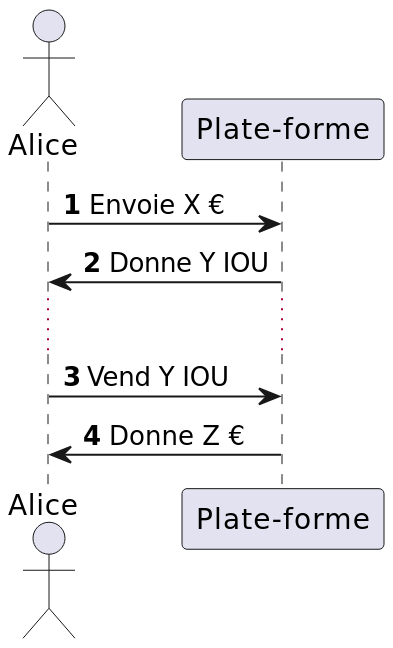
\includegraphics[scale = 0.25]{centralisation/img_plateformes/Achat-Vente.png}
        \label{fig:Order}
        \caption{Modélisation d'un Achat-Vente}
    \end{figure}
\end{frame}

\begin{frame}{Avantages et inconvénients}
    \begin{block}{Avantages}
        \begin{itemize}
            \item Diverses fonctionnalités.
            \item Utilisation simplifiée.
        \end{itemize}
    \end{block}
    \pause
    \begin{block}{Inconvénients}
        \begin{itemize}
            \item Sécurité et fiabilité relative au tiers.
            \item Gestion des données utilisateurs par le tiers.
            \item Fonctionnement interne opaque.
        \end{itemize}
        $\Rightarrow$ Confiance utilisateur/plate-forme.
    \end{block}
\end{frame}

%\begin{frame}{Fonctionnement opaque}
%    \begin{itemize}
%        \item Pas ou peu de documentation technique.
%        \item Code inaccessible.
%    \end{itemize}
%    \pause
%    \begin{block}{Ce que l'on sait}
%        \begin{itemize}
%            \item Fonctionnement en Order Book.
%            \item utilisation de bridges inter-blockchains.
%        \end{itemize}
%    \end{block}
%\end{frame}